\documentclass[11pt, a4paper, twocolumn]{article}

\title{\textbf{Object Detection in an Image}}
\author{Bruno de Almeida Silveira}
\date{October 2019}

\usepackage{url}
\usepackage{hyperref}
\usepackage{indentfirst}

\usepackage{booktabs}
\usepackage[table,xcdraw]{xcolor}

\usepackage{adjustbox}
\usepackage{lipsum}
\usepackage{caption}

\usepackage{amsmath}

\usepackage{graphicx}

\usepackage{xurl}

\graphicspath{ {./images-proposal/} }
\begin{document}

\maketitle

\section{Domain Background}

In 2016, Google released its first dataset with more than one object annotated by image \cite{google:1}, OpenImagesV1, which has around 1GB of images. This dataset was created and annotated by Google Inc under the CC BY 4.0 license.  In May of 2019, Google released a new version of this dataset \cite{google:2}, the fifth version, with a new Kaggle competition \cite{kaggle}, which was the inspiration for this project.

The problem of Object Detection in an image has some research on it, such as \cite{intro:1}, \cite{intro:2}, \cite{intro:3}, and \cite{intro:4}. A proper Object Detection model is the start of any image model recognition problem. So, this project intends to face it considering fundamental research for anyone who wants to work with images.

\section{Problem Statement}

The main challenge of this project is to create a model that identify and classifies all objects in a image.

The project intends to classify objects from 500 different classes correctly, and it is measured based on how many classes previously labeled it correctly predicts.

Like any classifier, it can be modeled as a Logistic Regression, some Support Vector Classifier (SVC) with some kernel, a Neural Network, among many other possible models. To this scope, Neural Networks are more applicable as a solution, even more, Deep Learning models.

This problem has many practical instances, like identifying objects in security footage; labeling a massive amount of photos automatically; automatically create a catalog for a retail company; and so many others.

\section{Datasets and Inputs}

The dataset used in this project is the same dataset provided in the Kaggle competition created by Google \cite{kaggle}. Google created the dataset labeling manually around 15 million of bounding boxes among 1.7 million images. Dataset is composed of a zip file with all images, a CSV that contains the position of each bounding box in each image and its class identifier, another CSV that maps each class identifier with a semantic class name, and a JSON file with the full hierarchical classes defined.

Google also divided the whole dataset using some stratified strategy to preserve the proportions of each class. More details could be found in the \cite{imgdataset}, the following table describes the division proposed.

\begin{table}[ht]
	\footnotesize
	\centering
	\caption{ \small Dataset division provided by Google }
	\label{table1}
	\begin{tabular}{@{}p{1.5cm}p{1.5cm}p{1.5cm}p{1.5cm}p{1.2cm}@{}}
		\rowcolor[HTML]{EFEFEF}
		& \multicolumn{1}{l}{\cellcolor[HTML]{EFEFEF}Train} & \multicolumn{1}{l}{\cellcolor[HTML]{EFEFEF}Validation} & \multicolumn{1}{l}{\cellcolor[HTML]{EFEFEF}Test} & \multicolumn{1}{l}{\cellcolor[HTML]{EFEFEF}Classes} \\
		Images & 1,743,042                                         & 41,620                                                 & 125,436                                          & -                                                      \\
		Boxes  & 14,610,229                                        & 303,980                                                & 937,327                                          & 600                                                    \\
	\end{tabular}
\end{table}

\section{Solution Statement}

To solve the problem, this project is going to use deep learning models, and it is going to use some transfer learning techniques in the state of the art of the Convolutional Neural Networks (CNNs) already designed \cite{cnns}, such as ResNet-N layers \cite{resnet}, Inception-V4 \cite{inception}, Xception \cite{xception} and Inception-ResNets \cite{inception}. The project is going to compare them with a couple of models tailored for this project, and see how all of them perform.

\section{Benchmark Model}

The benchmark models for this project are going to be the models created for Google's Kaggle competition \cite{kaggle}. So, the Leaderboard itself is going to be used as a benchmark \cite{leaderboard}. The top five achieve scores are 0.65887, 0.65337, 0.64214. 0.62221, and 0.60406.

\section{Evaluation Metrics}

The metric proposed by Google in the competition is the mean Average Precision (mAP) \cite{map}, a very didactic explanation about the metric could be found in here \cite{medium:1} and \cite{medium:2}.

The mAP metric could be defined as
{\centering
	\begin{equation*}
	mAP = \frac{\sum\limits_{c=1}^{C}AP_c} {C}
	\end{equation*}}
where $C$ value is the number of all categories (classes).

To understand $AP_c$, it must comprehend first what is $IoU$. $IoU$ is the Intersection over Union, and it is equal to the ratio of the area of intersection and area of the union of the predicted bounding box (created by the model) and Ground-truth bounding box (previously annotated).

\begin{figure}[ht]
	
	\centering
	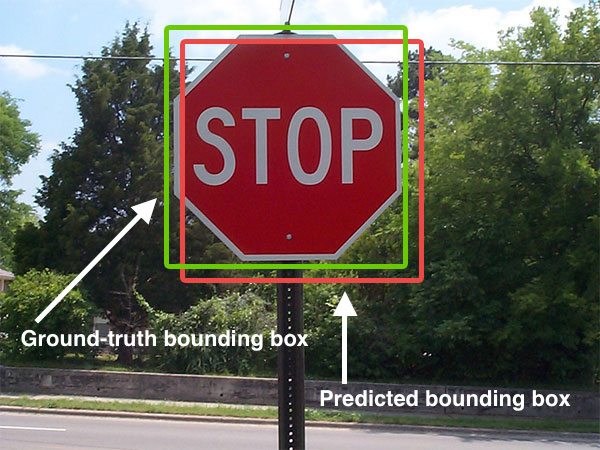
\includegraphics[width=0.4\textwidth]{iou_stop_sign.jpg}
	\caption{\scriptsize  Difference between a predict bounding box with a Ground-truth bouding box \cite{pyimage}}
	
\end{figure}

\begin{figure}[ht]
	
	\centering
	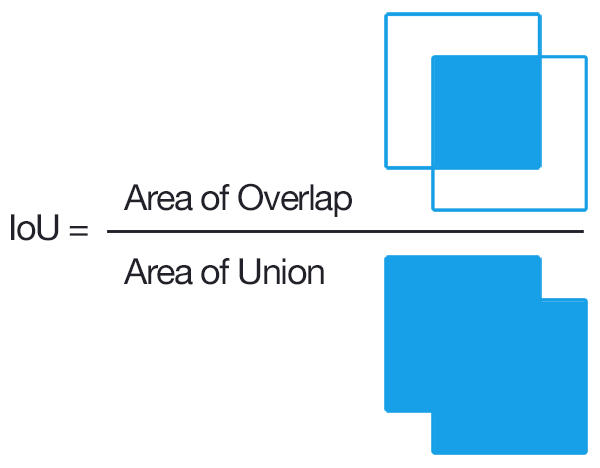
\includegraphics[width=0.4\textwidth]{iou_equation.png}
	\caption{\scriptsize IoU visual represented \cite{pyimage}}
	
\end{figure}

Here, it is going to define:
\begin{align*}
TruePositive\ \dot=&\ IoU > 0.5 \\
FalsePositive\ \dot=&\ IoU < 0.5 \\
         &or\ Duplicated PredictBoundingBox \\
FalseNegative\ \dot=&\ IoU > 0.5\ \\ 
&and \ WrongClassification
\end{align*}

With TP, TN, and FP defined, it is possible to create a Precision-Recall Curve, which defines a function that gives a precision based on the recall.

\begin{figure}[ht]
	
	\centering
	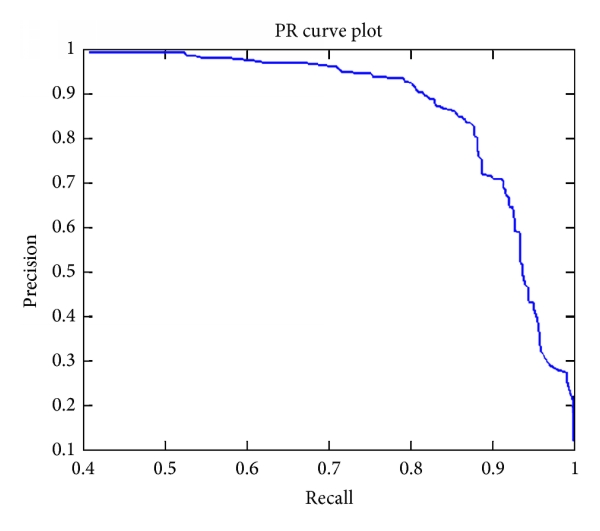
\includegraphics[width=0.5\textwidth]{precision-recall.png}
	\caption{\scriptsize Precision-Recall curve \cite{medium:1}}
	
\end{figure}

So by definition, $AP_c$ (Average Precision of some category c), is defined as an Area Under the Curve ($AUC$) of the Precision-Recall curve.

{\centering
\begin{equation*}
AP_c = \int_{0}^{1} p(r) dr
\end{equation*}
where $p(r)$ is the precision defined in function of recall.}

It is essential to retain that in this project it is going to be used $AP_{50}$ (which uses a threshold of 0.5 in $IoU$ to define $TP$), but other metrics could be evaluated, like, $AP_{75}$ (with $IoU$ threshold of 0.75) or $AP_{90}$ (with $IoU$ threshold of 0.90).

\section{Project Design}

(approx. 1 page)

In this final section, summarize a theoretical workflow for approaching a solution given the problem. Provide thorough discussion for what strategies you may consider employing, what analysis of the data might be required before being used, or which algorithms will be considered for your implementation. The workflow and discussion that you provide should align with the qualities of the previous sections. Additionally, you are encouraged to include small visualizations, pseudocode, or diagrams to aid in describing the project design, but it is not required. The discussion should clearly outline your intended workflow of the capstone project.

\bibliographystyle{unsrt}
\bibliography{references.bib}{}
\end{document}